\section{Experiments}

\subsection{Evaluation on d4rl datasets}

\textbf{Datasets construction.} In order to make a public comparison with other offline algorithms, we delay the dense reward based on the d4rl gym datasets. Specifically, we perform constant delay setting: we set a hyper-parameter $K$ as the delay interval which controls the sparsity of the delayed rewards. We set the delayed reward at equal intervals with $K$ as the un-discounted cumulative rewards of corresponding interval, the missing reward filled with 0, formally:

For a trajectory $\tau$ with length $T$, we set the delayed reward of time step $t$ as $r_t^{delay}$, where:

$$
\begin{aligned}
r_t^{delay} = \begin{cases}
0, \text{if} \ t \mod K \neq 0; \\
\sum_{i = t - K + 1}^t r_t, \text{otherwise}.
\end{cases}
\end{aligned}
$$

Such construction strategy introduce sparsity to delay rewards, meanwhile, it keeps the rule that for any trajectory in the original datasets, the un-discounted cumulative rewards keep constant before and after the operation, mathematically, we have:

$$
\sum_{t = 1}^{T} r_t = \sum_{t = 1}^{T} r_t^{delay}
$$

To facilitate intuitive and clear comparison of the delay reward construction method, visualization shows that:
\begin{figure}
    \centering
    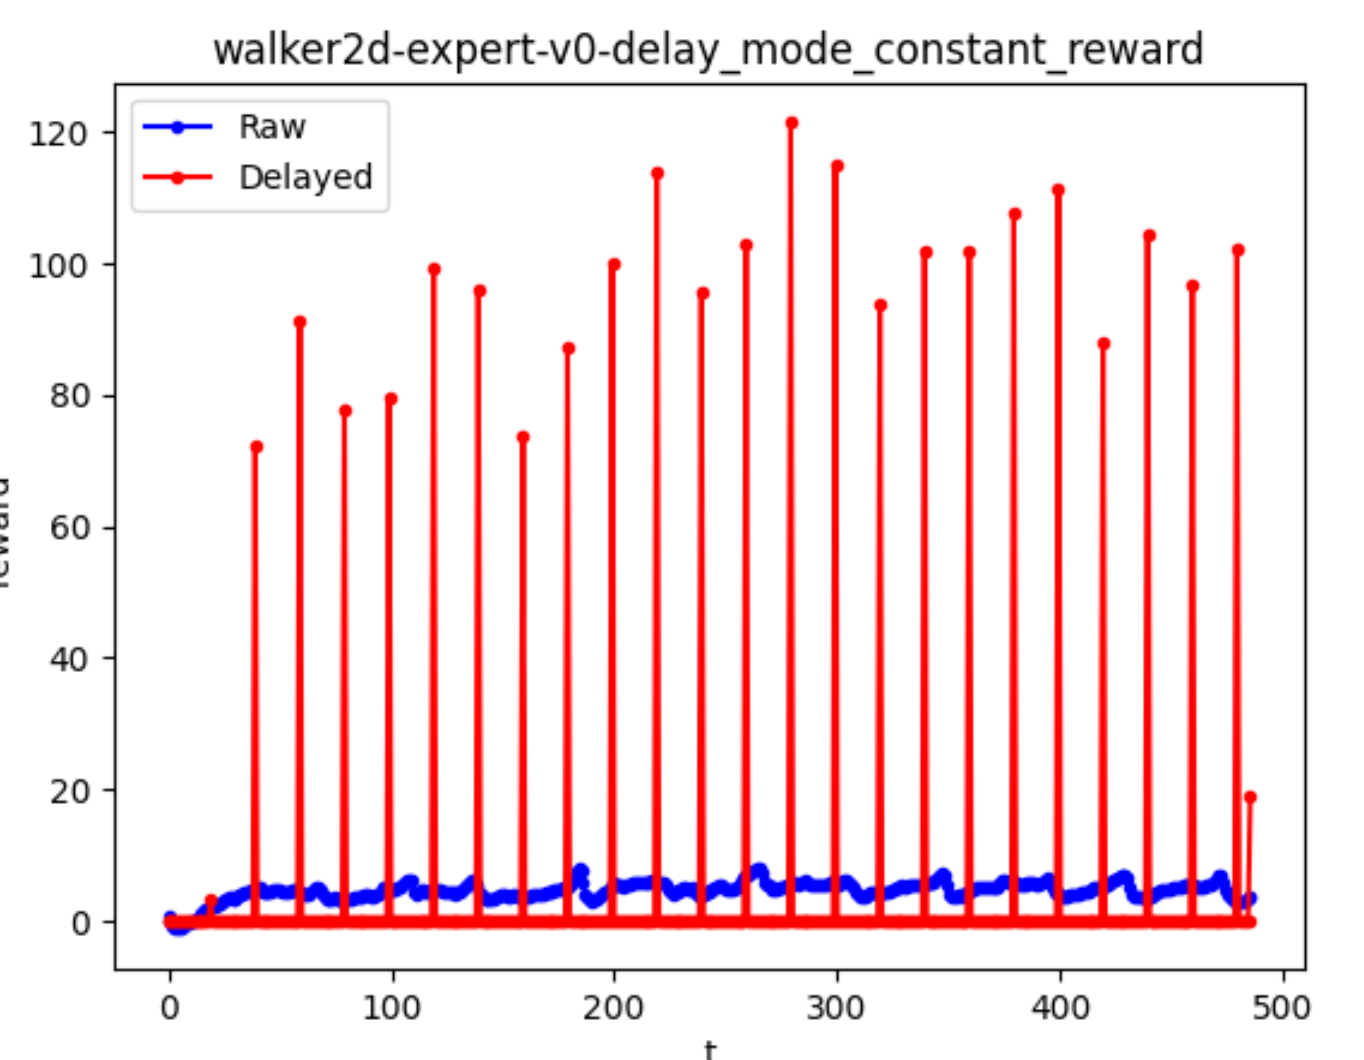
\includegraphics[width=0.95\textwidth]{assets/image.png}
    \caption{Delayed rewards xxx}
    \label{fig:fig1}
\end{figure}

\subsection{Evaluation on simulated datasets}


\subsection{Ablation Study}


